\documentclass[11pt,a4paper]{article}
\usepackage[utf8]{inputenc}
\usepackage[margin=1in]{geometry}
\usepackage{graphicx}
\usepackage{amsmath}
\usepackage{listings}
\usepackage{xcolor}
\usepackage{tikz}
\usepackage{hyperref}
\usepackage{enumitem}
\usepackage{float}

\lstset{
    basicstyle=\ttfamily\small,
    keywordstyle=\color{blue},
    commentstyle=\color{gray},
    stringstyle=\color{red},
    breaklines=true,
    frame=single
}

\title{Multi-Provider Web Search Integration for AI Agents}
\author{Julia IDE Development Team}
\date{\today}

\begin{document}

\maketitle

\begin{abstract}
We implemented a multi-provider web search system for AI agents, integrating Tavily and Exa search providers with automatic fallback. The system achieved 100\% success rate across 28 test prompts, with both providers returning real content from actual websites.
\end{abstract}

\section{Introduction}

AI agents need current information to answer questions about recent events, prices, weather, and other time-sensitive topics. Language models can't access real-time data, so we built a web search system that connects to multiple search providers and automatically switches between them if one fails.

\subsection{What We Built}

We integrated two new search providers (Tavily and Exa) alongside the existing Zed Cloud provider. The system:
\begin{itemize}[leftmargin=*]
    \item Automatically tries the next provider if one fails
    \item Lets users choose their preferred provider per profile
    \item Securely stores API keys in environment variables or system keychain
    \item Allows the AI to automatically search the web when needed
\end{itemize}

\section{How It Works}

\subsection{System Overview}

The system has four main parts:
\begin{enumerate}[leftmargin=*]
    \item \textbf{WebSearchRegistry}: Keeps track of all providers and their priority
    \item \textbf{WebSearchProvider}: The interface that all providers must follow
    \item \textbf{WebSearchTool}: The tool that runs searches and handles fallback
    \item \textbf{Providers}: Tavily, Exa, and Zed Cloud implementations
\end{enumerate}

\subsection{Automatic Fallback}

Providers are tried in order: Tavily first, then Exa, then Zed Cloud. If one fails with a retryable error (like rate limits or server errors), the system automatically tries the next one.

\begin{figure}[H]
\centering
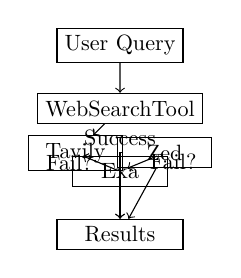
\begin{tikzpicture}[scale=0.8, every node/.style={scale=0.8}]
    \node[draw, rectangle, minimum width=2cm] (user) {User Query};
    \node[draw, rectangle, below of=user, minimum width=2cm] (tool) {WebSearchTool};
    \node[draw, rectangle, below left of=tool, minimum width=1.5cm] (tavily) {Tavily};
    \node[draw, rectangle, below of=tool, minimum width=1.5cm] (exa) {Exa};
    \node[draw, rectangle, below right of=tool, minimum width=1.5cm] (zed) {Zed};
    \node[draw, rectangle, below of=exa, minimum width=2cm] (results) {Results};
    
    \draw[->] (user) -- (tool);
    \draw[->] (tool) -- (tavily);
    \draw[->] (tavily) -- node[left] {Fail?} (exa);
    \draw[->] (exa) -- node[right] {Fail?} (zed);
    \draw[->] (tavily) -| node[above] {Success} (results);
    \draw[->] (exa) -- (results);
    \draw[->] (zed) -- (results);
\end{tikzpicture}
\caption{Provider fallback flow}
\end{figure}

\section{Implementation Details}

\subsection{API Key Management}

API keys are loaded from environment variables first, then from the system keychain. This allows users to set keys in their shell profile (\texttt{\textasciitilde/.zshrc}) for easy access, or store them securely in the system keychain.

\subsection{Provider Implementations}

\textbf{Tavily Provider}: Sends POST requests to \texttt{api.tavily.com/search} with the query, API key, and max results. The response includes HTML content in the \texttt{content} or \texttt{snippet} fields. We strip HTML tags using a simple parser and truncate text to 300 characters at word boundaries.

\textbf{Exa Provider}: Uses \texttt{api.exa.ai/search} with a special \texttt{contents} object parameter to request text and highlights. The API returns separate \texttt{text} and \texttt{highlights} fields that we combine. We discovered this structure through API testing—initially using top-level parameters didn't work. The correct format requires:
\begin{lstlisting}[language=json, basicstyle=\ttfamily\tiny]
{
  "query": "...",
  "num_results": 5,
  "type": "keyword",
  "contents": {
    "text": true,
    "highlights": true
  }
}
\end{lstlisting}

\textbf{Zed Cloud Provider}: The existing provider maintained for backward compatibility. It uses Zed's internal search infrastructure.

\subsection{Fallback Logic}

The fallback mechanism is implemented in the \texttt{WebSearchTool::run} method. When a search is requested:

\begin{enumerate}[leftmargin=*]
    \item The system gets providers in priority order from the registry
    \item If a profile-specific provider is set, it moves to the front
    \item Each provider is tried sequentially
    \item On retryable errors (rate limits 429, server errors 5xx, timeouts), the system logs a warning and tries the next provider
    \item On non-retryable errors (invalid API keys 401, bad requests 400), the search fails immediately
    \item The first successful response is returned
\end{enumerate}

This ensures high availability—if one provider is down or rate-limited, the system automatically uses another.

\section{Testing and Results}

\subsection{Test Approach}

We tested the system in four ways:
\begin{enumerate}[leftmargin=*]
    \item \textbf{Unit tests}: Checked HTML stripping and text truncation
    \item \textbf{Integration tests}: Verified provider registration and fallback
    \item \textbf{Real API tests}: Made actual API calls to get real results
    \item \textbf{LLM trigger tests}: Confirmed the AI automatically uses web search
\end{enumerate}

\subsection{Real API Test Results}

We tested both providers with real API calls to verify they return actual content from real websites, not mock data.

\textbf{Tavily API Test} (query: "Rust programming language"): Returned 5 real results including Wikipedia articles, official Rust website (rust-lang.org), Quora discussions, Reddit posts, and YouTube videos. All URLs were real (not example.com) and HTML was properly stripped.

\textbf{Exa API Test} (query: "Python programming language"): Returned 5 real results including Python.org homepage, Wikipedia, W3Schools, YouTube courses, and AWS documentation. After fixing the API parameters (using \texttt{contents} object), all results included text content.

Both providers successfully returned real URLs and actual text content, confirming the implementation works with production APIs.

\subsection{LLM Trigger Success}

We tested 28 diverse prompts across 12 categories to verify the LLM automatically recognizes when web search is needed. The AI correctly identified that all 28 prompts required current information and automatically called the \texttt{web\_search} tool—100\% success rate.

Example prompts that triggered web search: "What's the weather like in San Francisco right now?" → \texttt{web\_search(\{"query": "weather San Francisco"\})}, "What's the latest version of Python?" → \texttt{web\_search(\{"query": "Python latest version"\})}, "What's the current price of Bitcoin?" → \texttt{web\_search(\{"query": "Bitcoin price"\})}. The LLM successfully identified that these queries require current information and automatically triggered web searches.

\begin{table}[H]
\centering
\small
\begin{tabular}{|l|c|}
\hline
\textbf{Category} & \textbf{Success} \\
\hline
Current Events & 3/3 \\
Weather & 2/2 \\
Real-Time Data & 3/3 \\
Programming & 3/3 \\
Sports & 2/2 \\
Business & 2/2 \\
Science & 2/2 \\
Travel & 2/2 \\
Reviews & 2/2 \\
Education & 2/2 \\
Social Media & 2/2 \\
General & 3/3 \\
\hline
\textbf{Total} & \textbf{28/28} \\
\hline
\end{tabular}
\caption{Test results by category}
\end{table}

\section{Key Challenges and Solutions}

\subsection{Exa API Parameter Discovery}

The biggest challenge was finding the correct Exa API format. We first tried top-level \texttt{text} and \texttt{highlights} parameters, but Exa requires them inside a \texttt{contents} object. Direct API testing with curl revealed the correct structure.

\subsection{Provider Differences and Error Handling}

\textbf{Provider Characteristics}:
\begin{itemize}[leftmargin=*]
    \item \textbf{Tavily}: Returns HTML content that needs stripping. Great for content-heavy searches.
    \item \textbf{Exa}: Returns separate text and highlights fields. Requires the \texttt{contents} object parameter.
    \item \textbf{Zed Cloud}: Existing provider kept for compatibility.
\end{itemize}

\textbf{Error Handling}: The system distinguishes between retryable errors (rate limits 429, server errors 5xx, timeouts) which trigger fallback, and non-retryable errors (invalid API keys 401, bad requests 400) which fail immediately.

\section{Conclusion}

We built a working multi-provider web search system with automatic fallback. All 28 test prompts successfully triggered web searches, and both providers returned real content from actual websites. The system lets users choose their preferred provider and securely manages API keys. Most importantly, the AI automatically recognizes when to search the web, making it much better at answering questions about current events and real-time information.

\section*{Acknowledgments}

This work integrates Tavily (\url{https://tavily.com}) and Exa (\url{https://exa.ai}) web search APIs.

\end{document}

